% !TEX TS-program = pdflatexmk
\documentclass{./packages/optica-article}
\graphicspath{{images/}{practica1/images}}
\journal{opticajournal}

\usepackage{csvsimple}
\usepackage{siunitx}
\usepackage{physics}
\usepackage{booktabs}
\usepackage{tikz}

\usepackage{caption}
\usepackage{subcaption}
\usetikzlibrary{positioning}

\newcommand{\sinc}{\textrm{sinc}}
\newcommand\conv{\circledast}

% Set the article type
\articletype{Research Article}




\begin{document}

\title{Caracterización de sistemas de formación de imágenes}

\author{Adriana Mamani Lazarte\authormark{1} Alex G. Recuenco\authormark{1}, y Carlos España Castaño\authormark{1}}

\address{\authormark{1}Universidad Complutense de Madrid, Madrid, CP 28040, España}

%Índice,
\tableofcontents
\newpage

\section{Introducción}
En esta práctica vamos a caracterizar un sistema de formación de imágenes mediante la determinación experimental de su función de transferencia de modulación (MTF). Para ello utilizaremos un método directo (el test de barras) y un método indirecto (el test de borde). La MTF nos aportará información sobre el rango de frecuencias espaciales, estimar su resolución y el contraste de la imagen a estudiar.

Para tal fin anteriormente mencionado tuvimos que entender la respuesta a un impulso, la función de transferencia de modulación de la imagen, el poder distinguir si nuestro sistema es lineal e invariante con respecto a su desplazamiento y sus descripciones.




\section{Marco práctico}
El sistema cuya MTF mediremos consiste en un objetivo de microscopio con apertura numérica $\textrm{NA} = 0,25$ y un aumento $10\times$ (F10),
y una cámara CCD con un tamaño de píxel de $s=4,65 \unit{\micro\meter}$.
Las imágenes captadas por la cámara se visualizarán en la pantalla del PC.
A continuación se detallará el procedimiento práctico realizado utilizando los dos métodos de medición de la MTF.


\subsection{Medida de MTF mediante el test de barras (método directo)}\label{sec:metodo-directo}

Este método consiste en medir el contraste para varios conjuntos de barras de distintas frecuencias de la imagen obtenida. El contraste de un conjunto de barras nos da directamente el valor la MTF del sistema para la frecuencia de ese conjunto. Representando los contrastes frente a las frecuencias obtenemos la función MTF(u), y realizando un ajuste de los datos se puede determinar la frecuencia de corte.

Se utilizó el test USAF 1951 (Fig.~\ref{fig:usaf1951}) como imagen general en la que se captaron fotografías de  distintos conjuntos de barras de la diapositiva de la Fig.~\ref{fig:usaf1951} presentada a continuación. Se controla la exposición para obtener los colores grises en cada muestra de imagen sin sobre-exposición.

\begin{figure}[h]
	\centering
	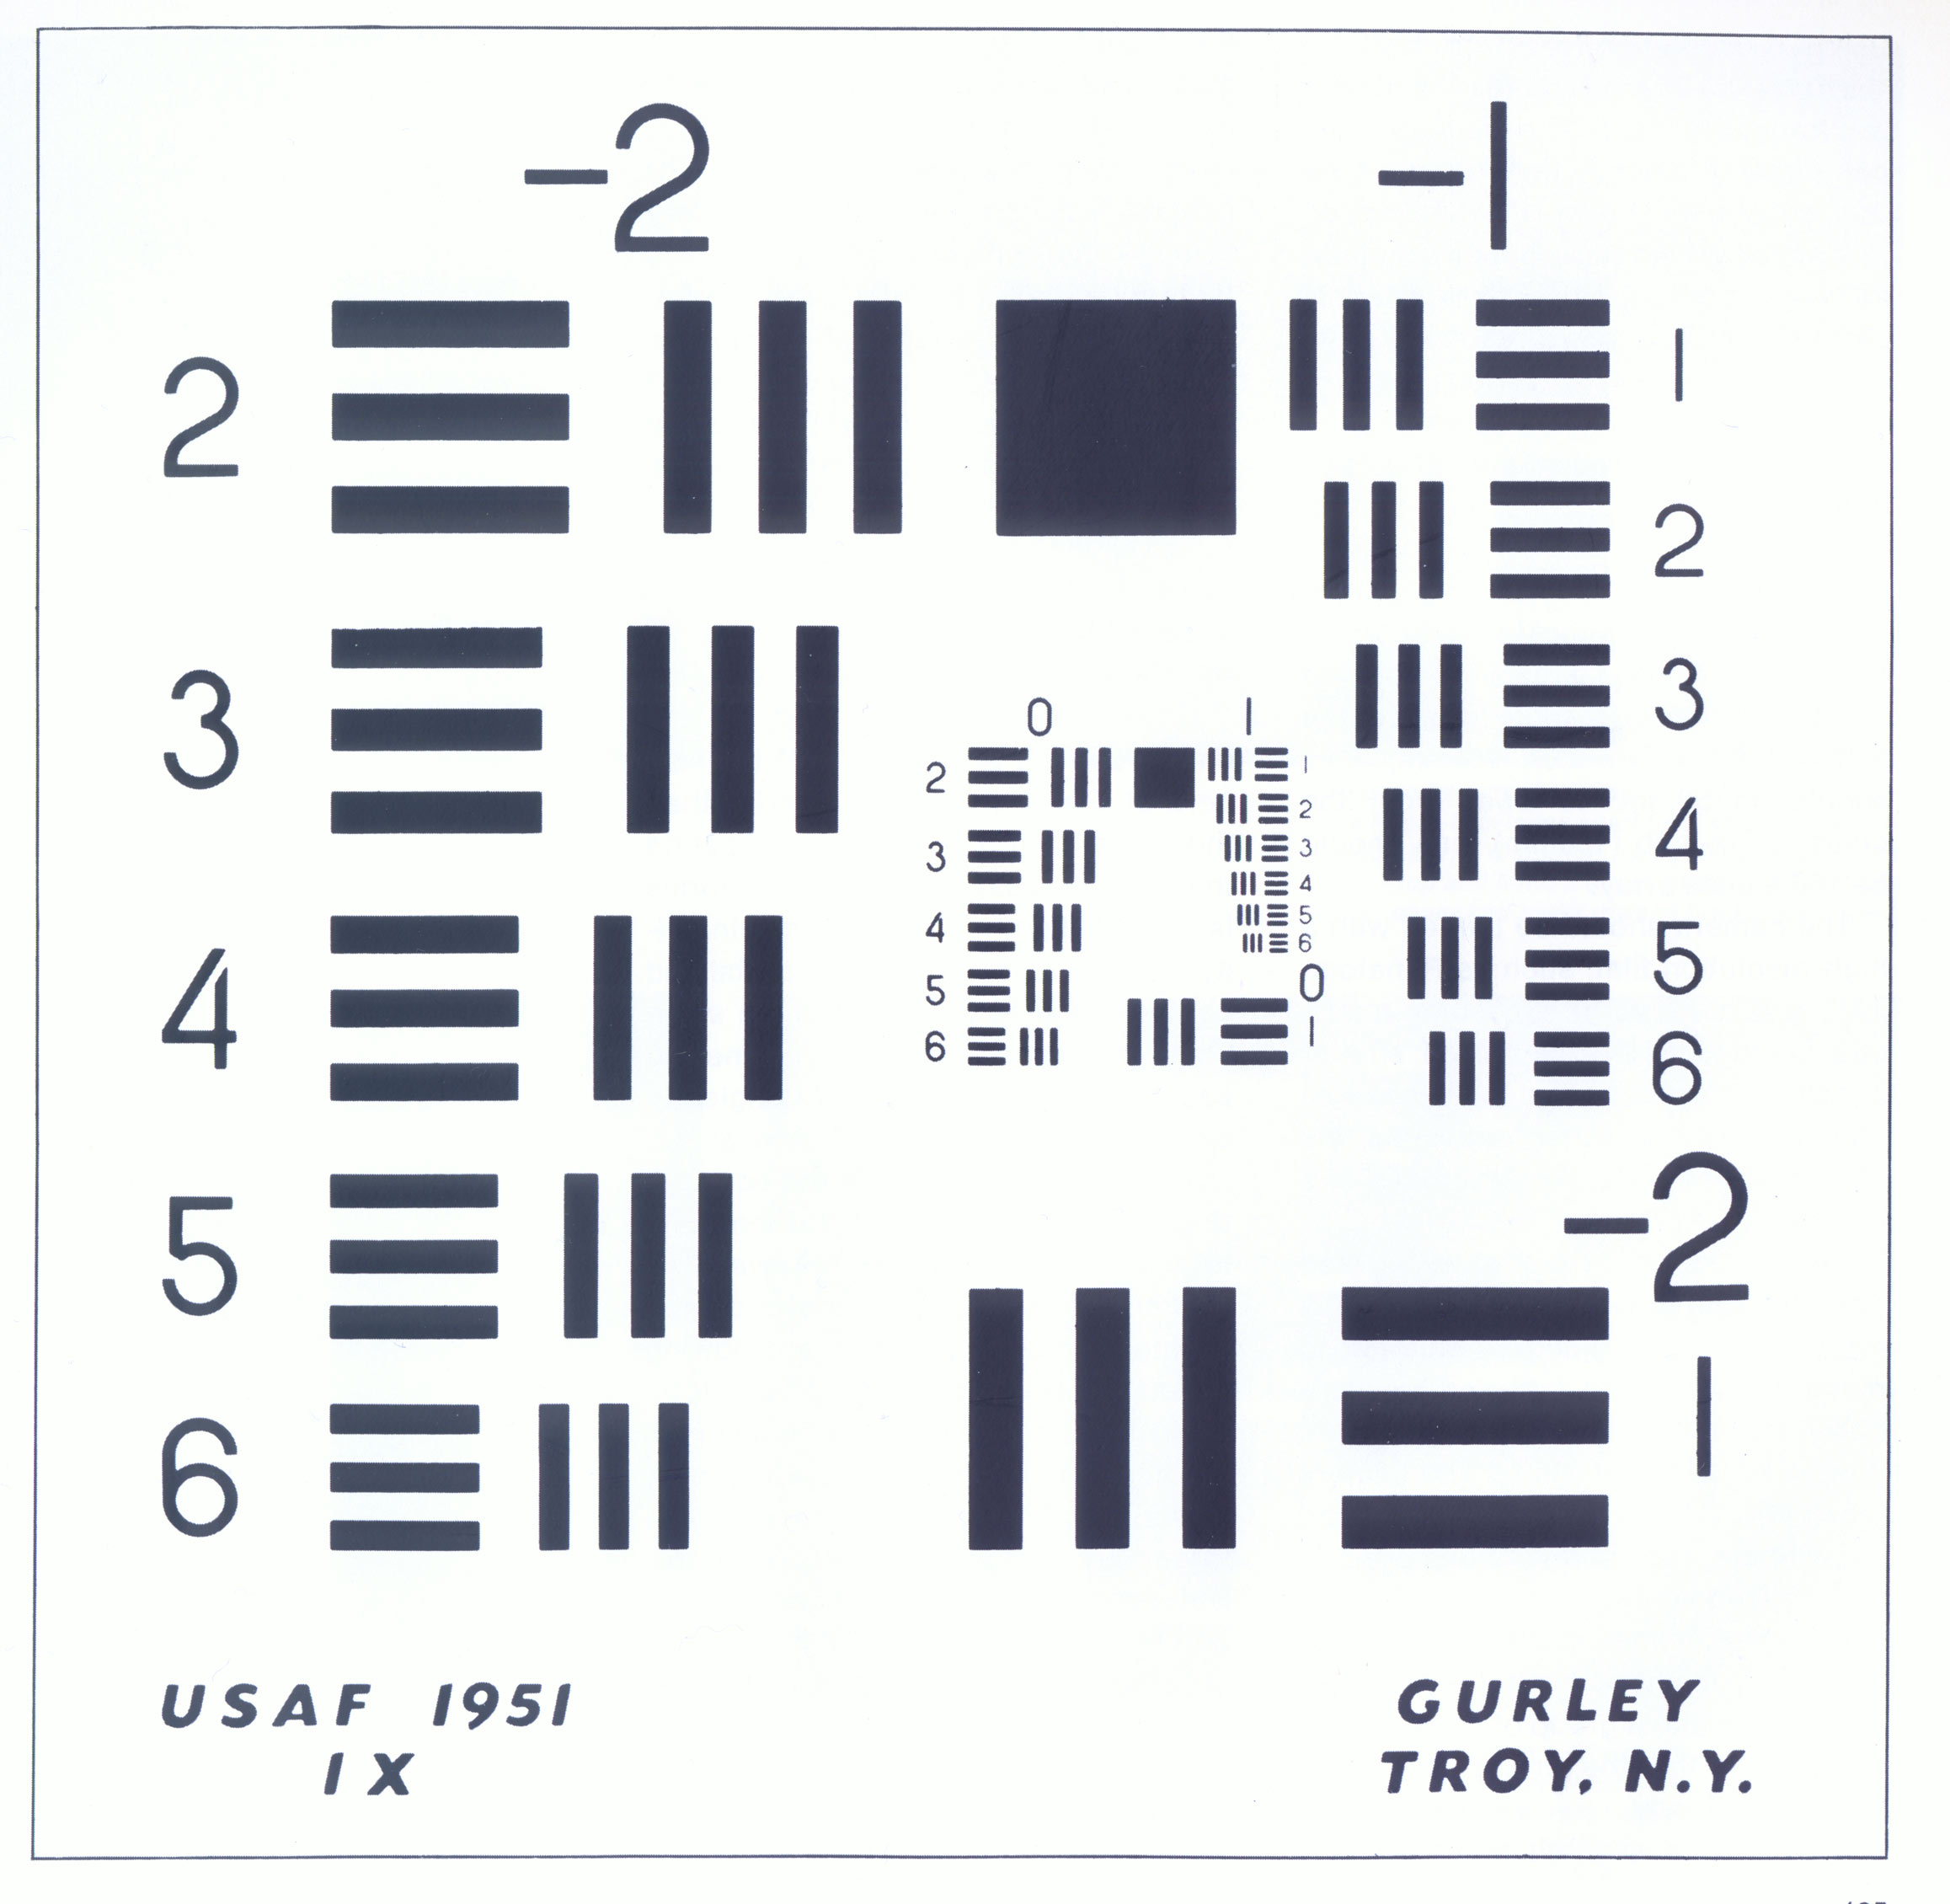
\includegraphics[scale=0.08]{testusaf1951}
	\caption{Test USAF 1951.}\label{fig:usaf1951}
\end{figure}

A través de las imágenes tomadas (figura ~\ref{fig:group:usaf}) se obtiene un perfil ortogonal a las rendijas de contraste, para cada una de las distintas imágenes. Los resultados se discutirán en la sección~\ref{sec:mtf-directo} del apartado de Resultados experimentales. Este perfil es obtenido mediante un software diseñado en la plataforma de MATLAB.

\begin{figure}[h]
\centering
\begin{subfigure}[t]{0.576\textwidth}\centering
	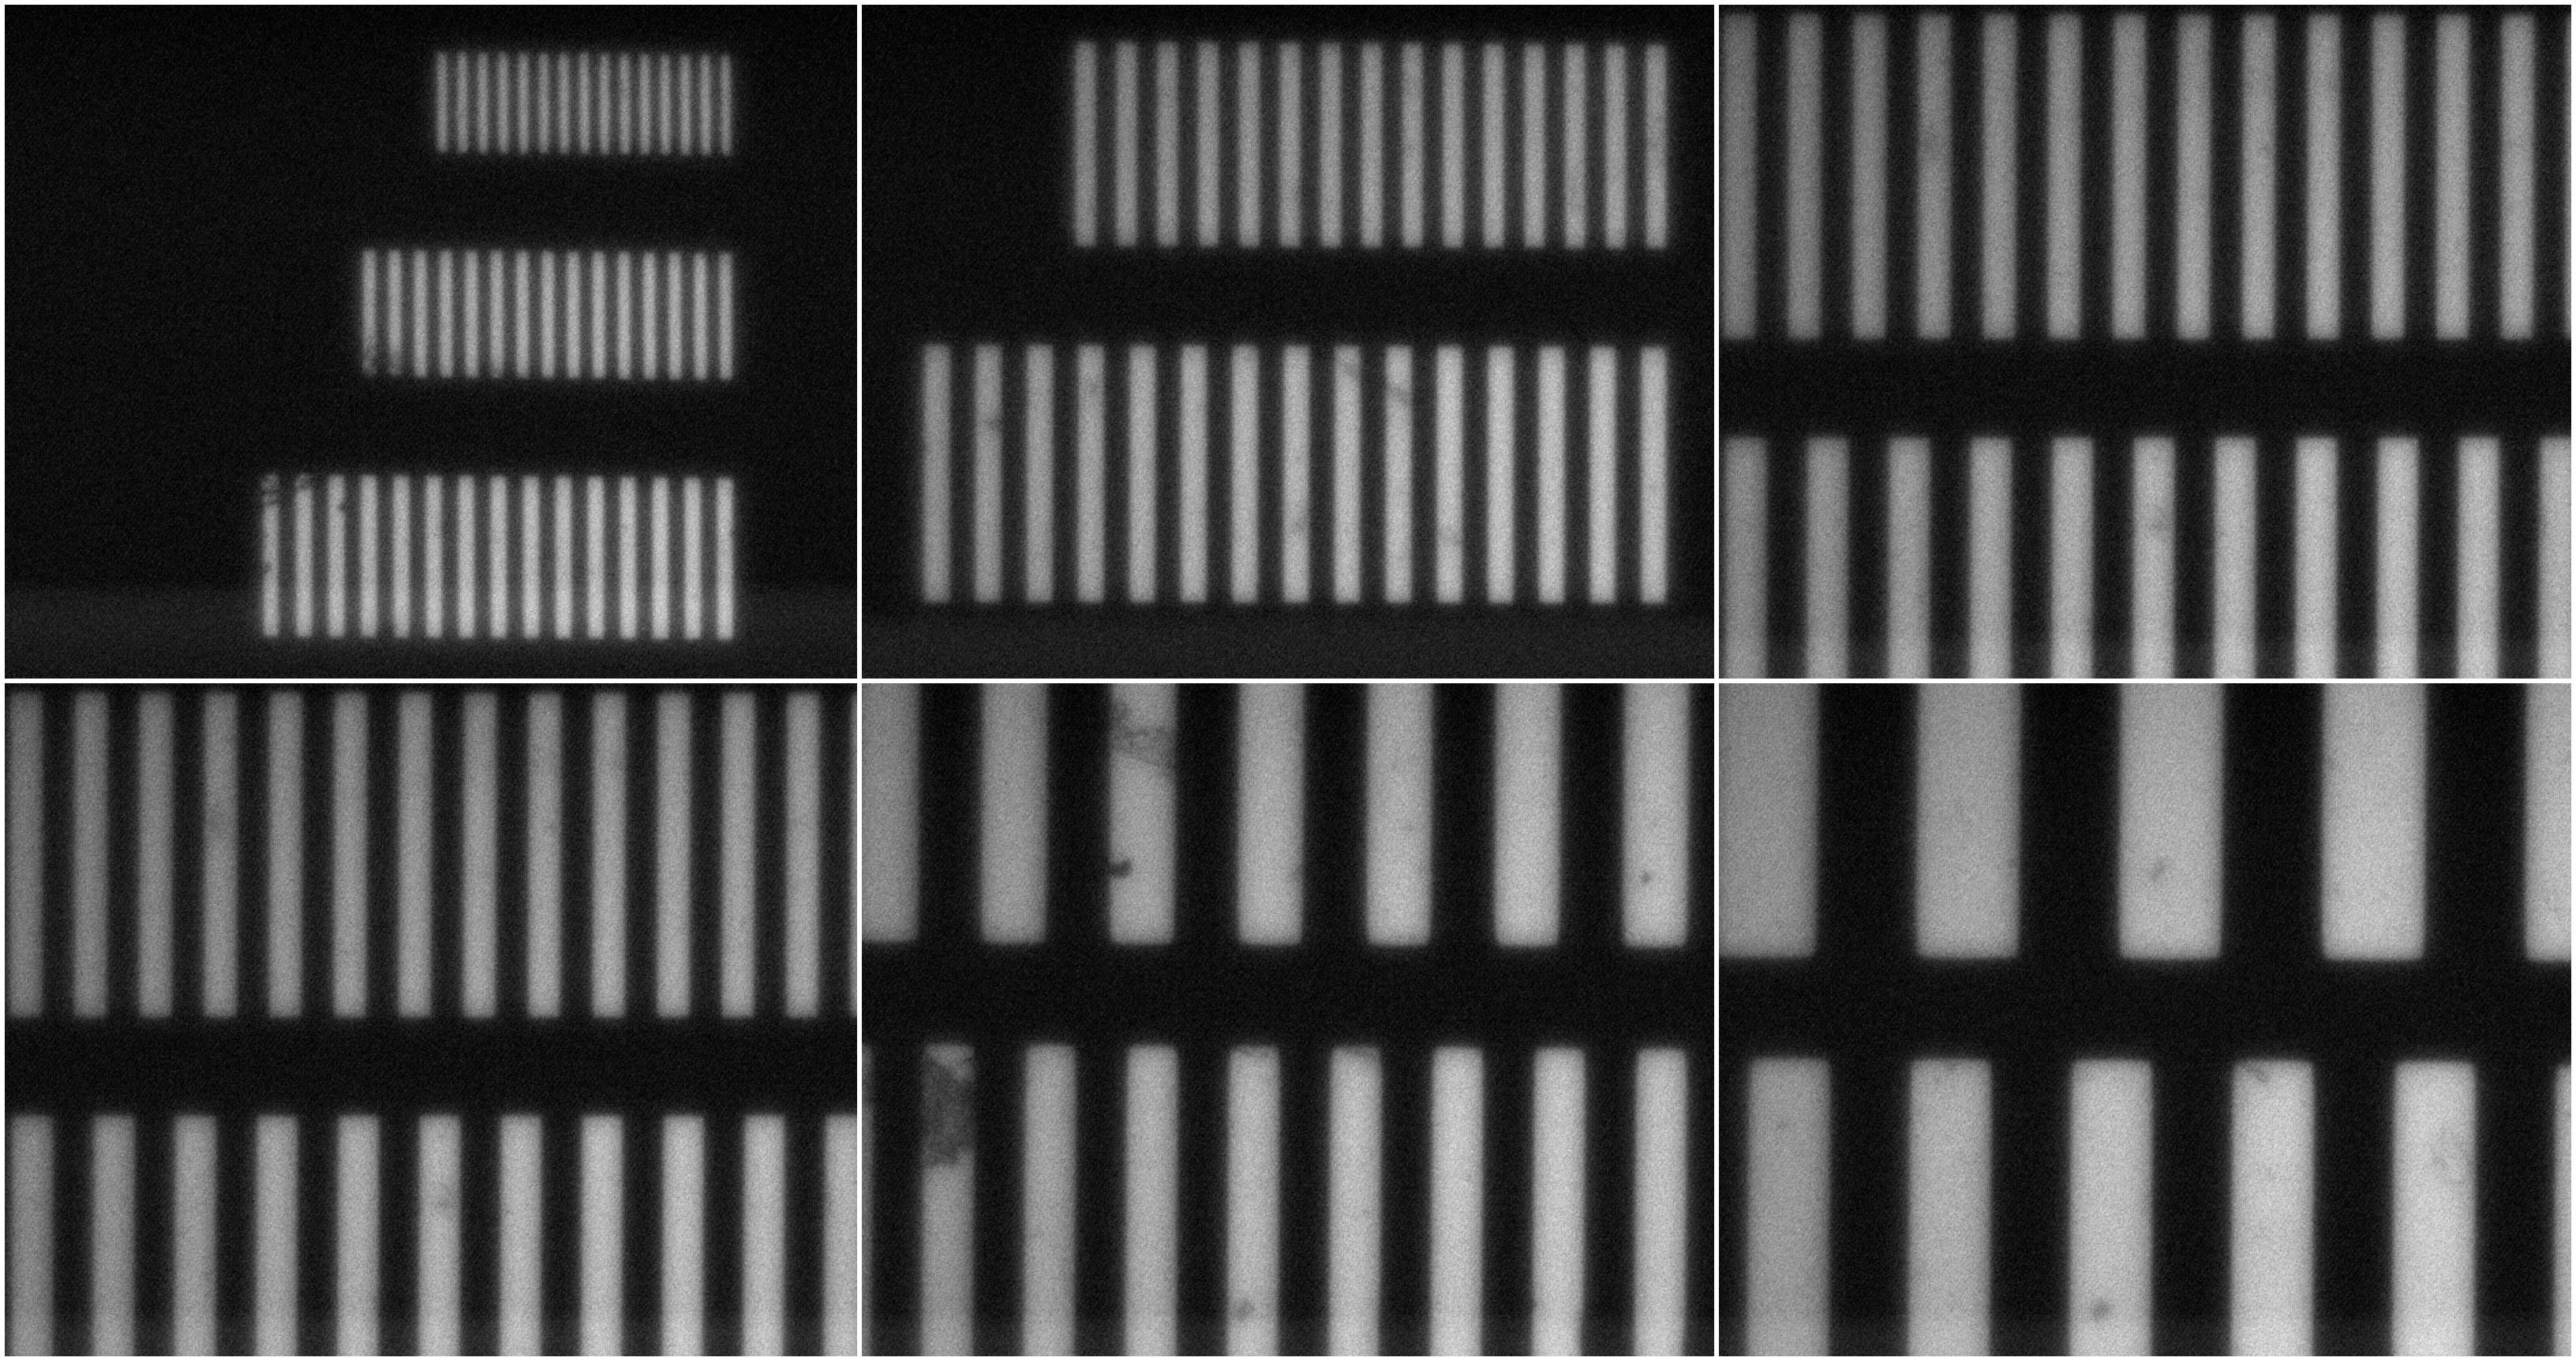
\includegraphics[width=\textwidth]{/imaglineas.jpg}
	\caption{Imágenes tomadas del test de USAF Fig.~\ref{fig:usaf1951} para la medida del MTF directo}\label{fig:images:example}
\end{subfigure}
\,
\begin{subfigure}[t]{0.4\textwidth}\centering
	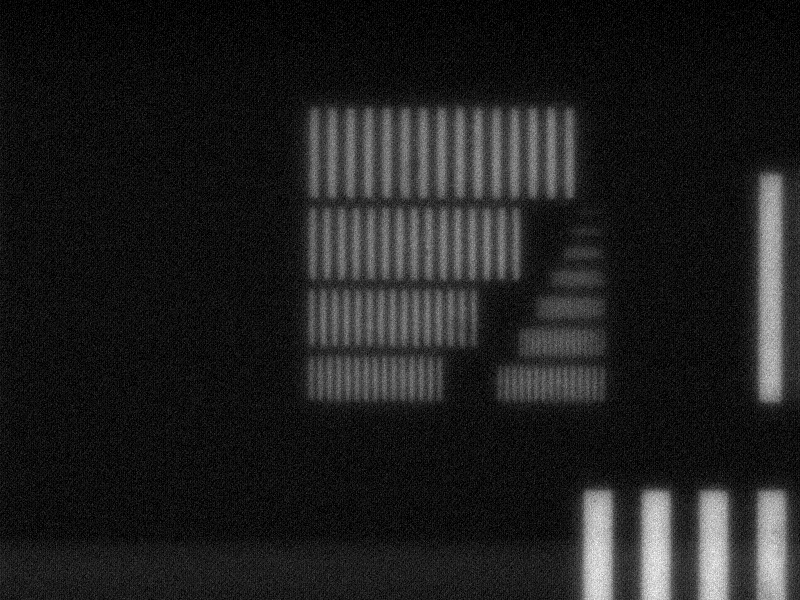
\includegraphics[width=\textwidth]{smallest_lines}
	\caption{Foto tomada durante la práctica de las líneas centrales del test USAF 1951}\label{fig:usafpic}
\end{subfigure}
\caption{Fotos tomadas durante la práctica}\label{fig:group:usaf}
\end{figure}


Del perfil de intensidad se obtienen el contraste y la frecuencia a partir del perfil de un segmento de líneas es el siguiente: Se obtiene dos posiciones tan distantes como se pueda de dos mínimos de las barras. Se mide la distancia en píxeles entre ellas ($x_{\max} - x_{\min} $) y se cuenta el número de periodos entre ellas, lo que nos permite calcular el periodo en píxeles como $T = \flatfrac{(x_{\max} - x_{\min)} }{N_{\textrm{periodos}}}$. A continuación,  se toma los máximos y mínimos de altura $y_{\max}$, $y_{\min}$.

El contraste se ha obtenido a partir de la expresión:
\nopagebreak
\begin{equation}
	C = \frac{y_{\max} - y_{\min}}{y_{\max} + y_{\min}}.
	\label{eq:contraste}
\end{equation}

La frecuencia se calcula como:
\nopagebreak
\begin{equation}
	\nu = \frac{1825}{T}\ \textrm{ciclos/mm}\label{eq:frecuencia}
\end{equation}

Donde el periodo, $T$, de acuerdo a la gráfica del perfil obtenida en el estudio de cada imagen.



\subsection{Medida de la MTF mediante el test de borde (método indirecto)}\label{sec:description:indirecto}

Se obtiene la imagen de la misma manera que el apartado anterior, pero esta vez de una única barra que abarque el campo completo de visión como se puede ver en la Fig.~\ref{fig:perfil:img}. Con la imagen del borde obtenida, obtenemos su perfil de intensidad (la "respuesta a una escalón" o SR) y posteriormente su derivada ("line spread function", o LSF). La transformada de Fourier de la LSF nos da la MTF del sistema, a partir de la cual estimamos su frecuencia de corte.

Esto es debido a que la función $\delta(x)$ es la derivada de la step function, $s(x)$. Como distribución, podemos usar este hecho para calcular la LSF, encontrando primero la respuesta a un borde. Realizando una estimación de la derivada, podemos obtener la MTF de una manera más rápida.

Los resultados se presentarán en la sección de resultados correspondiente.





\section{Resultados experimentales}\label{sec:resultados}

\subsection{Resultados medidas de la MTF mediante el test de barras (método directo)}\label{sec:mtf-directo}

Un ejemplo de perfil estudiado para un conjunto de barras se muestra en la figura \ref{fig:perfil:example}.

\begin{figure}
	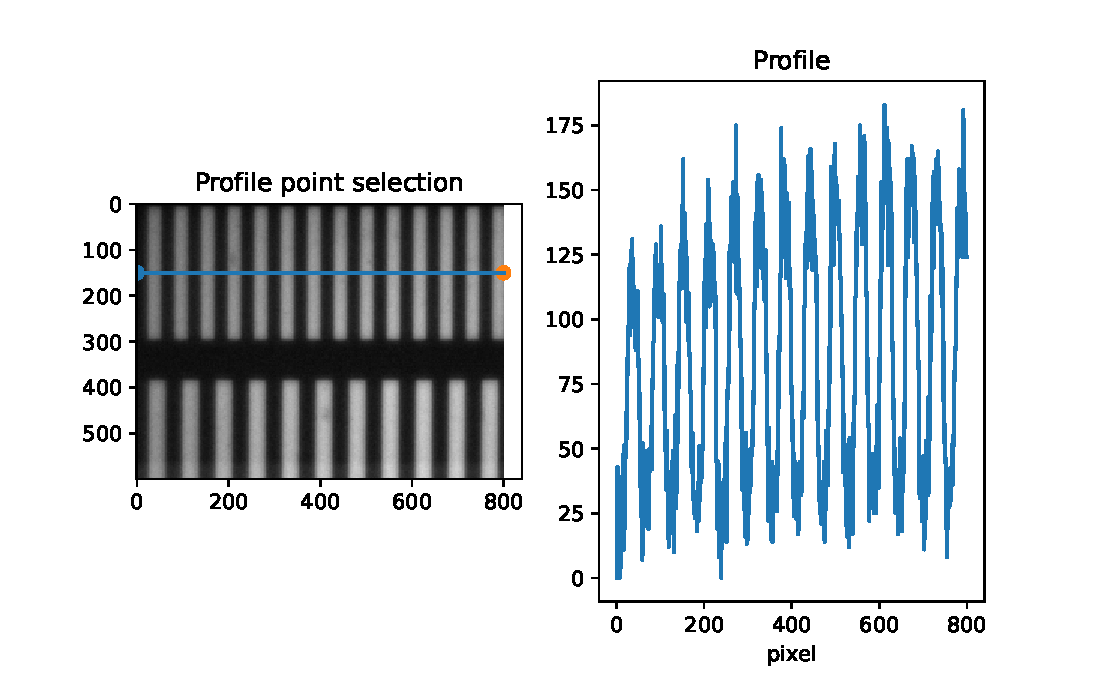
\includegraphics[width=\textwidth]{profile-lines.pdf}
	\caption{Perfil de un segmento de líneas}\label{fig:perfil:example}
\end{figure}

En la tabla \ref{table:perfilintensidad} se recogen las medidas tomadas de los perfiles de intensidad para distintos conjuntos de barras, así como la frecuencia (líneas/mm) y el contraste calculados según las ecuaciones ~\ref{eq:frecuencia} y ~\ref{eq:contraste}.

\begin{table}[hbp]
	\centering
	\csvautotabular[
		table head=\toprule%
		Barras & $y_{\min} (px)$ & $y_{\max} (px)$ & Contraste & $x_{\min} (px)$ & $x_{\max} (px)$ & N Periodos & periodo (px) &  $\flatfrac{\textrm{ciclos}}{\textrm{mm}}$%
		\\\midrule%
	]{practica1/MTF/Profiles.csv}
	\caption{Datos de los perfiles de intensidad. $y$: intensidad. $x$. El contraste se ha obtenido a partir de la ecuación~\ref{eq:contraste}. La frecuencia se ha obtenido a través de la ecuación~\ref{eq:frecuencia}. Como se obtienen los periodos se explica visualmente en la Fig.~\ref{fig:perfil:example}}%
	\label{table:perfilintensidad}
\end{table}

Representando el contraste de la imagen frente a la frecuencia (cliclos/mm) se obtiene la MTF del sistema (figura $~\ref{fig:mtf-directo}$).

\begin{figure}
    \centering
    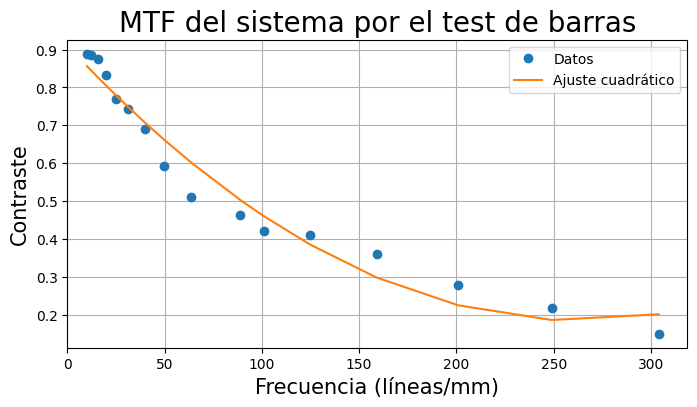
\includegraphics[scale=0.5]{MTF-directo.png}
    \caption{MTF del sistema obtenida mediante el test de barras (método directo). Ajuste: $C = 1,05 \cdot 10^{-5} u^2 + 1,52 \cdot 10^{-3} u + 0,91$, donde u es la frecuencia y C el contraste.}
    \label{fig:mtf-directo}
\end{figure}

El sistema se comporta como un filtro pasa baja. Las frecuencias superiores a la frecuencia de corte, con una transferencia teóricamente nula, no son captadas a la salida del sistema. En nuestro estudio comprobamos que los conjuntos de barras de más de 250-300 líneas/mm ya no aparecían resueltos en la imagen, aunque la presencia de ruido impedía visualizar frecuencias mayores. 

La frecuencia de corte del sistema según la teoría es mayor. En la sección ~\ref{sec:cuestion:mtf} se muestra la gráfica de la MTF del sistema calculada mediante un modelo teórico. Según predice la teoría, esta MTF se puede aproximar a una función cuadrática. Se realizó por tanto un ajuste cuadrático de los datos experimentales, obteniendo la ecuación $C = 1,05 \cdot 10^{-5} u^2 + 1,52 \cdot 10^{-3} u + 0,91$, con un coeficiente $R^2$ de $0,964$. Esta función tiene su mínimo en un valor de la frecuencia de $u = 263$ líneas/mm, el cual dista mucho de la frecuencia de corte teórica de 1000 líneas/mm (sección ~\ref{sec:cuestion:mtf}). Esta discrepancia puede deberse al ruido, de manera que se pueden haber tomado valores de los máximos y mínimos de los perfiles que no correspondían con los de la señal de interés (la imagen) sino con picos de ruido. Tomando un valor de los máximos y de los mínimos promedio se eliminaría este problema y probablemente se obtendría un mejor ajuste de los datos.

Este método permite la medida directa de la respuesta del sistema a cada frecuencia determinada, lo cual puede ser de utilizada cuando se requiera un comportamiento específico a frecuencias concretas. En la siguiente sección utilizaremos otro método que permite calcular la MTF del sistema experimentalmente para más frecuencias de una forma más rápida.





\subsection{Resultados Medida de la MTF mediante el test de borde (método indirecto)}\label{sec:resultados:indirecto}


En la figura ~\ref{fig:perfil} se muestran los resultados de manera gráfica para mejor interpretación.
\begin{figure}[hptb]
	\centering
	\begin{subfigure}[t]{0.35\textwidth}
		\centering
		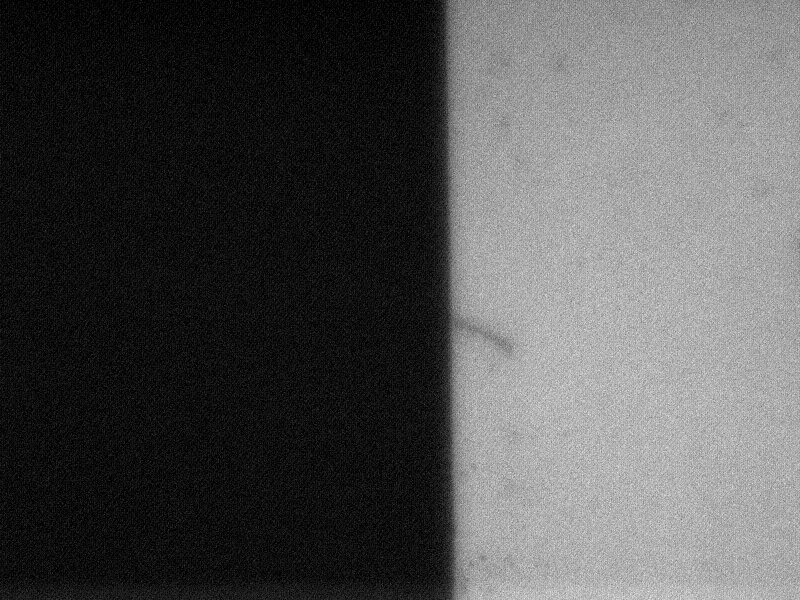
\includegraphics[height=4cm]{edge_large_line}
		\caption{Imagen de una franja amplia}\label{fig:perfil:img}
	\end{subfigure}
	\quad
	\begin{subfigure}[t]{0.60\textwidth}
		\centering
		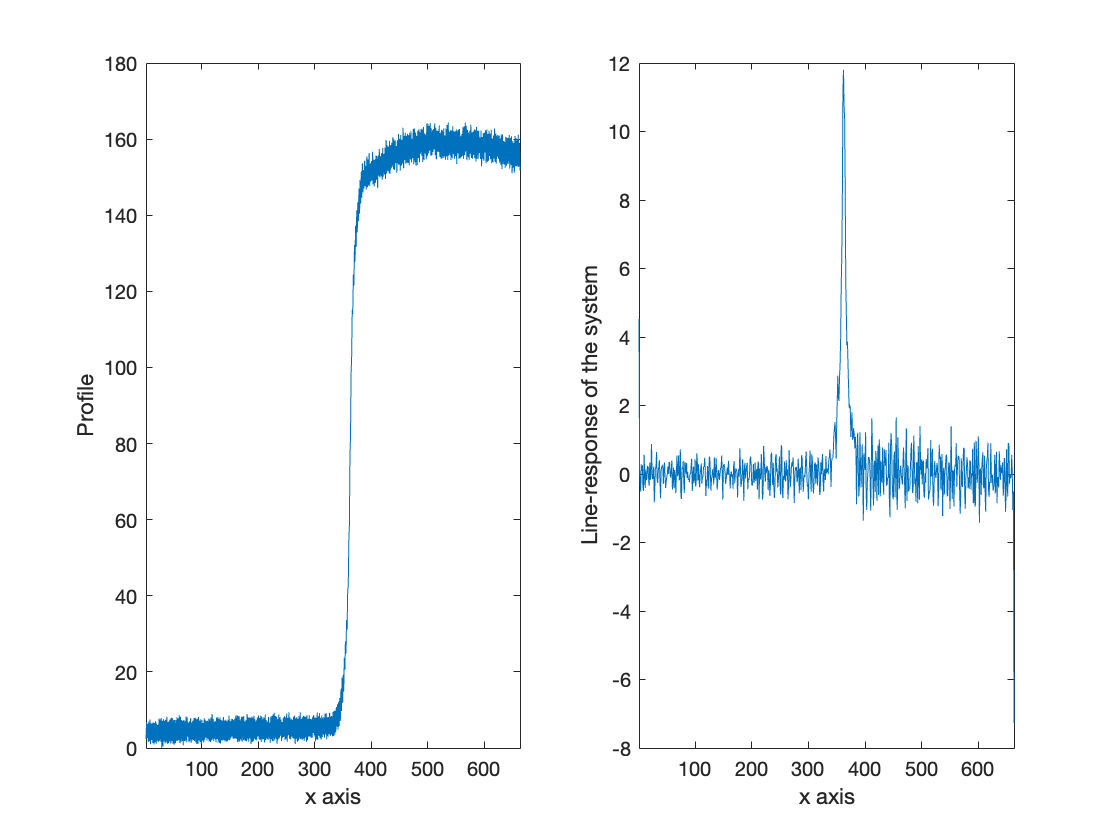
\includegraphics[width=\textwidth, height=4cm]{/lsf_edge.png}
		\caption{Perfil de intensidad de píxeles en una línea horizontal (izqda) y la derivada de este perfil (drcha). La derivada es igual al LSF}\label{fig:perfil:graph}
	\end{subfigure}
	\caption{Perfil de intensidad de una franja grande utilizada para el método indirecto para obtener el MTF, como se describe en la sección~\ref{sec:description:indirecto}}\label{fig:perfil}
\end{figure}

Mediante un programa de MATLAB podemos calcular fácilmente la transformada de Fourier de la LSF mostrada en la figura ~\ref{fig:perfil:graph} (gráfica derecha). Esta TF es la MTF del sistema (figura ~\ref{fig:mtf-indirecto}).

\begin{figure}
    \centering
    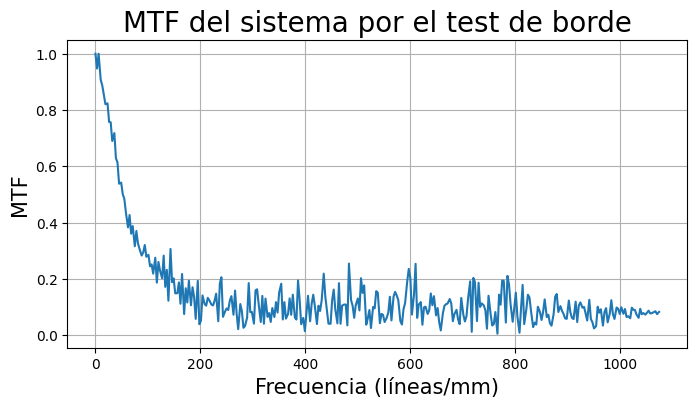
\includegraphics[scale=0.5]{/MTF-indirecto.png}
    \caption{MTF del sistema obtenida mediante el test de borde (método indirecto)}
    \label{fig:mtf-indirecto}
\end{figure}

La frecuencia de corte estimada con este método indirecto se sitúa entre 200 y 300 líneas/mm. Ambos métodos arrojan resultados parecidos, aunque no concuerdan con los predicho por la teoría. Comparando las gráficas de ambos métodos (figuras ~\ref{fig:mtf-directo} y ~\ref{fig:mtf-indirecto}), vemos que el rango de frecuencias que pasan por el sistema es aproximadamente el mismo. Sin embargo, la caída del valor de la MTF es más acusada en el caso de este último método del test de borde. Esto evidencia que en las medidas de los máximos y mínimos de los perfiles de intensidad en el método directo se tomaron los valores más extremos del perfil, obteniéndose un contraste mayor que el contraste real de la imagen. Habiendo tomado como máximo un valor promedio de todos los máximos, y lo mismo para los mínimos, las dos gráficas habrían salido probablemente más parecidas aún.

El método del test de borde tiene la ventaja respecto al método de barras de permitirnos visualizar la MTF para un mayor rango de frecuencias. Este puede resultar más útil que el método directo para caracterizar sistemas en un rango completo de frecuencias de forma rápida. 






\section{Cuestiones}

\subsection{Sea $H_{c}(u)$ la función de transferencia de un sistema para luz coherente. Escribir la relación entre $H_{c}(u)$ y la función de transferencia del mismo sistema para luz incoherente, $H_{i}(u)$.}\label{sec:cuestion:incoherente}

Cuando la luz incidente es coherente, la imagen resultante se obtiene añadiendo linealmente la amplitud compleja. Sin embargo, cuando la iluminación es idealmente incoherente, la iluminación es linear en la intensidad de la onda incidente. Por ello, en el caso ideal donde la correlación de fase es cero para distintas posiciones, se obtiene que~\cite[p.~132--134]{goodman1996introduction}.
\nopagebreak
\begin{equation}
	I_{i}(u,v) = \kappa \iint_{-\infty}^{\infty}\abs{h(u - \xi, v- \eta)}^{2} I_{g}(\xi, \eta) \dd \xi \dd \eta.
\end{equation}

Por lo tanto, la función $H_{i}(u)$ se puede obtener con el esquema descrito en Fig.~\ref{fig:transformacion}. Básicamente, haciendo la transformación inversa para obtener $h_{c}$, luego multiplicando está con su conjugada, obteniendo $h_{i}$, donde $i$ denota intensidad. Y al realizar la transformada inversa obtenemos el resultado.

\begin{align*}
	H_{i}(u)
	 & = TF\{h_i\}
	= TF\left\{ h_{c} \cdot h^{*}_{c}\right\}
	= TF\left\{ h_{c} \cdot h^{*}_{c}\right\}
	= TF\left\{ TF^{-1}\{H_{c}\} \cdot {TF^{-1}\{H_{c}\}}^{*}\right\}
	\\
	 & = H_{c} \conv H^{*}_{c}. %
	% Numerar sólo la última equación.
	\addtocounter{equation}{1}\tag{\theequation} \label{eq:incoherent-conv}
\end{align*}

\begin{figure}[htpb]
	\begin{center}
		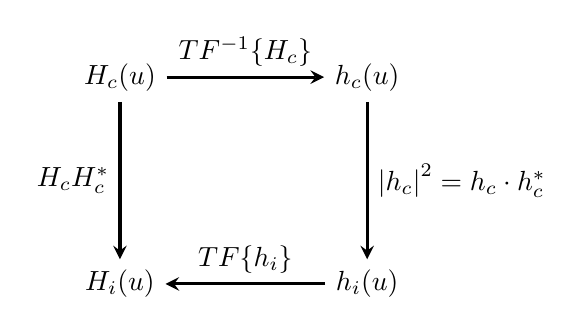
\begin{tikzpicture}[line width=0.4mm, >=stealth]
			\def \n {5}
			\def \radius {3cm}
			\def \margin {8} % margin in angles, depends on the radius

			\node (H) at (0,0) {$H_{c}(u)$};
			\node[right=2cm of H] (h) {$h_{c}(u)$};
			\node[below=2cm of h] (hi) {$h_{i}(u)$};
			\node[below=2cm of H] (Hi) {$H_{i}(u)$};
			\draw[->] (H) -- (h) node[pos=0.5, anchor=south] {$TF^{-1}\{H_{c}\}$};
			\draw[->] (h) -- (hi) node[pos=0.5, anchor=west] {$\abs{h_{c}}^{2} = h_{c} \cdot h^{*}_{c}$};
			\draw[->] (hi) -- (Hi) node[pos=0.5, anchor=south] {$TF\{h_{i}\}$};
			\draw[->] (H) -- (Hi) node[pos=0.5, anchor=east] {$H_{c} \conv H^{*}_{c}$};
		\end{tikzpicture}
	\end{center}
	\caption{Diagrama del proceso para obtener la PTF de intensidad\ref{sec:cuestion:incoherente} }\label{fig:transformacion}
\end{figure}


\subsection{Para un sistema parecido al usado en la práctica:}\label{sec:cuestion:mtf}
	\begin{enumerate}
		\item Estimar la frecuencia de corte de la cámara CCD, $u_{c}^{(CCD)}$, en líneas por milímetro.
		
	    La resolución de la cámara CCD está limitada por su tamaño de píxel. La frecuencia límite de un conjunto de barras que es capaz de resolver es aquella en la que cada barra tiene un tamaño de 1 px. La frecuencia de este conjunto de barras es la frecuencia de corte de la cámara, y viene dada por:
	    
	    \begin{equation}
	        u_c^{(CCD)} = \frac{1}{2s} = 108 \flatfrac{ciclos}{mm}
	    \end{equation}
		
		Donde $s=4,65 \mu m$ es el tamaño del píxel. Esta frecuencia corresponderá a la imagen formada por el objetivo, la cual está aumentada x10. Esto se tendrá en cuenta para calcular la MTF del sistema entero. La $u_^{(CCD)}$, no obstante, se da como la frecuencia de la imagen, que hace de objeto para la cámara.
		
		\item Estimar la frecuencia de corte $u_{c}^{(Obj)}$ del objetivo $10\times$ para luz incoherente (la longitud de onda media $\lambda=500\,\unit{\nano\metre}$).
		
		La frecuencia de corte del objetivo viene dada por:
		
		\begin{equation}
		    u_c^{(Obj)} = \frac{2 NA}{\lambda} = 1000 \flatfrac{ciclos}{mm}
		\end{equation}
		
		Donde $NA=0,25$ es la apertura numérica del objetivo en el espacio objeto. Al igual que para el cálculo de $u_^{(CCD)}$, esta frecuencia se da como la frecuencia del objeto, que en este caso es el propio objeto del sistema, la diapositiva del test USAF 1951.
		
		\item Tomando estos valores y suponiendo que la PSF del objetivo y de la cámara se aproximan por la función $|\sinc(ax)|^2$, dibujar la MTF de cada uno de los elementos y del sistema compuesto.
		
		La MTF de cada elemento es la transformada de Fourier (TF) normalizada de la PSF $|\sinc(ax)|^2$. El parámetro ''a'' será la frecuencia de corte $a=u_c^{(Obj)}$ en el caso del objetivo. Para la cámara, $a=10 u_c^{(CCD)}$, puesto que la imagen formada por el objetivo (el objeto de la cámara) está aumentada x10. De esta manera obtenemos la MTF(u) de la cámara en función de las frecuencias (u) de la diapositiva del test USAF 1951, igual que la MTF(u) del objetivo. Así, la MTF del sistema será el producto las MTF de los dos elementos del mismo. 
		
		\begin{enumerate}
		    \item MTF del objetivo y la cámara CCD:
		    
		    La TF de $|\sinc(ax)|^2$ es la función triangular con un factor $\flatfrac{1}{|a|}$:
    		    \begin{equation}
    		        \wedge(u)= \left\{ \begin{array}{lcc}
                 \frac{1}{|a|}(1-|\frac{u}{a}|) &   si  & |u| \leq 1 \\
                 \\ 0 &  si & |u| \geq 1 \\
                 \end{array}
                \right.
		    \end{equation}
		    
		    La MTF para cada elemento es $MTF(u) = \frac{\wedge(u)}{\wedge(0)}$, y $\wedge(0) = \frac{1}{|a|}$. Por tanto, para el objetivo quedaría:
		        \begin{equation}
    		       MTF^{(Obj)}(u)= \left\{ \begin{array}{lcc}
                     1-|\frac{u}{1000}| &   si  & |u| \leq 1 \\
                     \\ 0 &  si & |u| \geq 1 \\
                     \end{array}
                    \right.
		    \end{equation}
		    
		    Y para la cámara CCD: 
		    	\begin{equation}
    		       MTF^{(CCD)}(u)= \left\{ \begin{array}{lcc}
                     1-|\frac{u}{1080}| &   si  & |u| \leq 1 \\
                     \\ 0 &  si & |u| \geq 1 \\
                     \end{array}
                    \right.
		    \end{equation}
		    
		    Véase que la MTF de la cámara, $\wedge^{(CCD)}(u)$, está en función de las frecuencias del objeto del sistema (la diapositiva USAF 1951), ya que vamos a obtener la MTF del sistema multiplicando las dos MTF.
		    
		    
		    \item MTF del sistema y representación gráfica
		    
		    La MTF del sistema viene dada por la ecuación ~\ref{eq:mtf-teorica}. En la figura ~\ref{fig:mtf-teorica} se muestran las MTF de los elementos y la del sistema conjunto.
		    
		    \begin{equation}
		        MTF(u) = MTF^{(Obj)}(u) \cdot MTF^{(CCD)}(u)
		    \end{equation}
		    \begin{equation}
		        MTF(u)= \left\{ \begin{array}{lcc}
                     (1-|\frac{u}{1080}|)(1-|\frac{u}{1000}|) &   si  & |u| \leq 1 \\
                     \\ 0 &  si & |u| \geq 1 \\
                     \end{array}
                    \right.
                    \label{eq:mtf-teorica}
		    \end{equation}
		        
		    
		    \begin{figure}
		        \centering
		        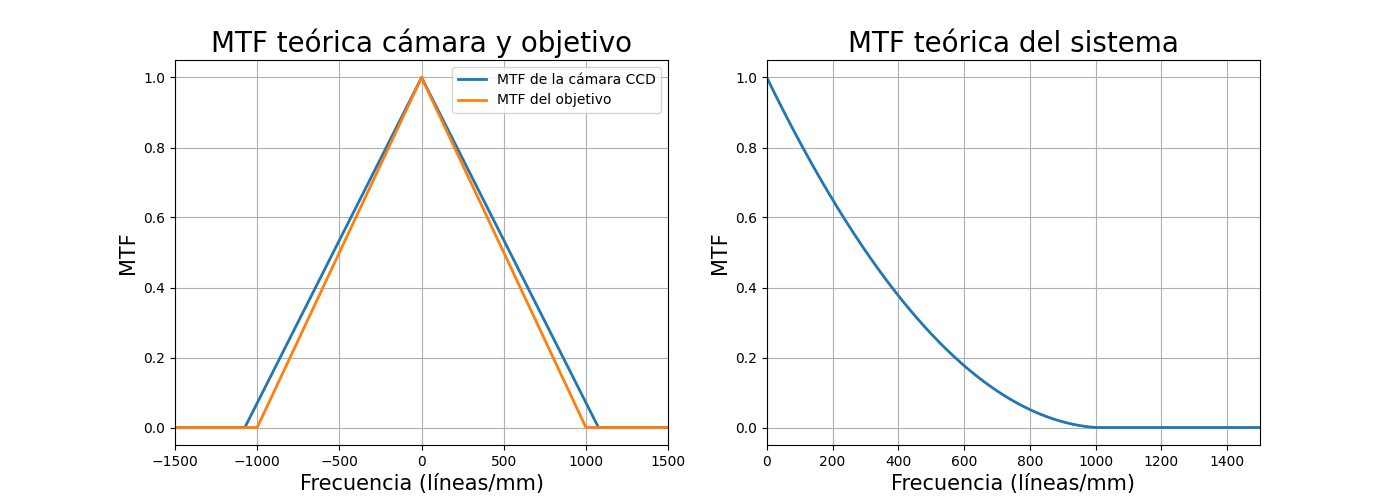
\includegraphics[scale=0.45]{/MTF-teorica.png}
		        \caption{MTF teóricas de los elementos del sistema y del sistema compuesto}
		        \label{fig:mtf-teorica}
		    \end{figure}
		    
		    Desarrollando el producto obtenemos la ecuación cuadrática que mencionamos en el estudio del método directo, aunque con distintos coeficientes:
		    
		    \begin{center}
		        \begin{math}
		        MTF(u) = 9,3 \cdot 10^{-7} u^2 + 1,9 \cdot 10^{-3} u + 1
		        \end{math}
		    \end{center}
		    
		    La MTF del sistema tiene la misma forma que las obtenidas experimentalmente, aunque con una frecuencia de corte mayor. Esta viene determinada por la frecuencia de corte del objetivo (1000 líneas/mm), que es la más restrictiva de las frecuencias de corte de los dos elementos. Esto significa el tamaño de píxel de la cámara es lo suficientemente grande como para adquirir todas las frecuencias espaciales de las imágenes formadas por el objetivo. 
		    
		    Que la frecuencia de corte teórica sea tan alta respecto a la del experimento (1000 líneas/mm frente a unas 200-300 líneas/mm) puede deberse a diversas causas relacionadas con la no idealidad de la realidad experimental: ruido, aberraciones, etc., que no se han tenido en cuenta en el cálculo teórico. Concretamente, el ruido de las imágenes impidió diferenciar máximos y mínimos en los perfiles de intensidad de conjuntos de barras de mayor frecuencia, aunque estos fueron bien resueltos por la cámara CCD. 
		    
		\end{enumerate}
		
	\end{enumerate}


\subsection{Aplicar usando el pluging Deconvolutionlab2 y Image J dos métodos de convolución: Regularized Inverse Filter y Richardson-Lucy a una imagen test obtenida por un sistema con una PSF conocida y diferentes tipos de ruido: Gauss y Poisson.}


\begin{figure}[hbp]
	\centering
	\begin{subfigure}[t]{0.45\textwidth}\centering
		\centering
		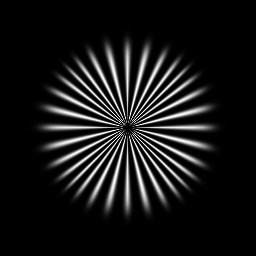
\includegraphics[width=\textwidth]{Simulation deconvolution/ref.jpg}
		\caption{Imagen referencia test original}\label{fig:ref}
	\end{subfigure}
	\hfill
	\begin{subfigure}[t]{0.45\textwidth}\centering
		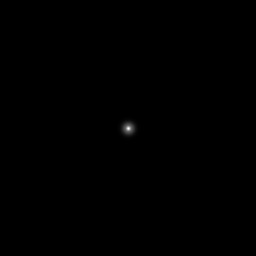
\includegraphics[width=\textwidth]{Simulation deconvolution/psf.jpg}
		\caption{Imagen PSF}\label{fig:psf}
	\end{subfigure}
	\caption{Imagen usada para la simulación con Deconvolutionlab2 y Image J, y el PSF del sistema de captura simulado}\label{fig:image:ref-psf}
\end{figure}
 
 Simulamos tomar fotos de la imagen de referencia (Fig.~\ref{fig:ref}) con un systema con Point Spread Function (PSF) del sistema simulado (Fig.~\ref{fig:psf}). Queremos estudiar distintos tipos de ruido simulado y que algoritmos de de-noising actúan mejor para reducir este ruido.

 Realizamos las siguientes simulaciones de observación con ruido. (Las imágenes obtenidas se ven en Fig.~\ref{fig:convolutions})

\begin{enumerate}
    \item \emph{Noiseless convolution} (convolución sin ruido)
    \item \emph{Simulation with noise-Gauss} (convolución con ruido Gaussiano. $\mu=0$, $\sigma=0.1$, y $0.01$
    \item \emph{Simulation with noise-Poisson} (Convolución con ruido Poisson 0.01, 10 y 0.0001.
    \item Aplicar a las imagenes anteriores \emph{Regularized Inverse filter (RIF)}: =0.01, =1.y Richardson-Lucy (RL) algorithm con 10 y 50 iteraciones. Probamos 100 iteraciones para una caso y comparar con 50 iteraciones
\end{enumerate}

Al realizar el tratado de las imágenes a las cuales se le aplicó ruido, podemos observar a ante la aplicación de un RIF menor con un número de iteraciones menor, se visualiza una recuperación de la imagen mejor filtrada, en cambio, a mayor número de los parámetros anteriormente mencionados la imagen coge más ruido, hasta degradándose en sus colores originales.

Por otro lado, la deconvolución de Richardson-Lucy, al ser procedimiento iterativo para recuperar una imagen subyacente que ha sido añadida ruido por una función de dispersión de puntos conocida, tiene mejores resultados en su filtrado.

\begin{figure}[hbp]
	% Esto no se hace asi con hfill y \, ... pero no me acuerdo como
	\begin{center}
		\,\hfill
		\begin{subfigure}[t]{0.25\textwidth}\centering
			\centering
			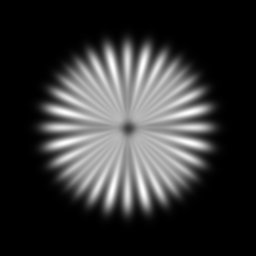
\includegraphics[width=\textwidth]{Simulation deconvolution/ref_conv}
			\caption{Convolution noiseless}\label{fig:sim:conv}
		\end{subfigure}
		\,\hfill
		\begin{subfigure}[t]{0.25\textwidth}\centering
			\centering
			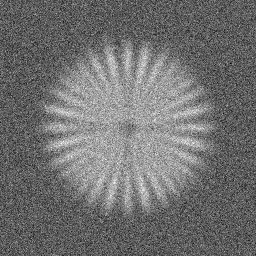
\includegraphics[width=\textwidth]{Simulation deconvolution/ref_ng_0.1}
			\caption{Convolution NG. $Mean=0$, $Stdev=0.1$}\label{fig:sim:ng0.1}
		\end{subfigure}
		\hfill
		\begin{subfigure}[t]{0.25\textwidth}\centering
			\centering
			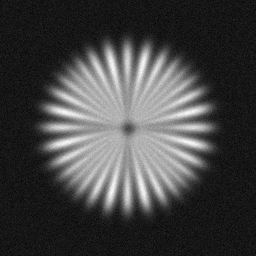
\includegraphics[width=\textwidth]{Simulation deconvolution/ref_ng_0.01}
			\caption{Convolution NG. $Mean=0$, $Stdev=0.01s$}\label{fig:sim:ng0.01}
		\end{subfigure}
		\hfill\,
		\\
		\hfill\,
		\begin{subfigure}[t]{0.25\textwidth}\centering
			\centering
			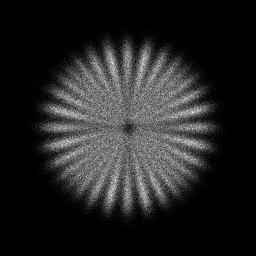
\includegraphics[width=\textwidth]{Simulation deconvolution/ref_np_0.01}
			\caption{Convolution NP 0.01}\label{fig:sim:np0.01}
		\end{subfigure}
		\hfill
		\begin{subfigure}[t]{0.25\textwidth}\centering
			\centering
			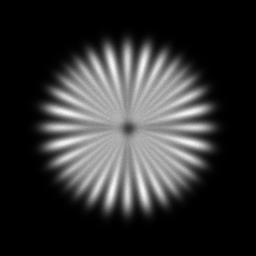
\includegraphics[width=\textwidth]{Simulation deconvolution/ref_np_0.0001}
			\caption{Convolution NP 0.0001}
		\end{subfigure}
		\hfill
		\begin{subfigure}[t]{0.25\textwidth}\centering
			\centering
			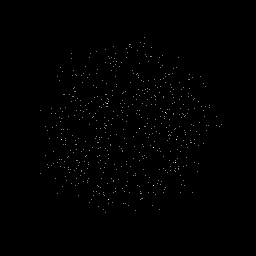
\includegraphics[width=\textwidth]{Simulation deconvolution/ref_np_10}
			\caption{Convolution NP 10}
		\end{subfigure}
		\hfill\,
		\caption{Simulación de la figura ~\ref{fig:image:ref-psf} con distintos tipos de ruido}\label{fig:convolutions}
	\end{center}
\end{figure}


\begin{figure}[hbp]
	\centering
	\begin{tabular}[t]{l c c c c}
		Original Image                                                                  & RIF 0.01 & RIF 1 & RL 10 & RL 50 \\
		Fig.~\ref{fig:sim:conv}                                                         &
		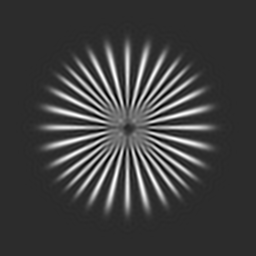
\includegraphics[scale=0.25]{Simulation deconvolution/ref_conv/RIF_0.01.png}    &
		
\includegraphics[scale=0.25]{Simulation deconvolution/ref_conv/RIF_1.png}       &
		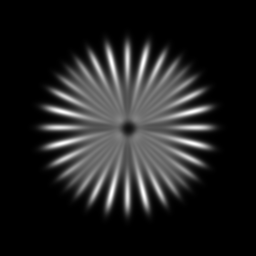
\includegraphics[scale=0.25]{Simulation deconvolution/ref_conv/RL_10.png}       &
		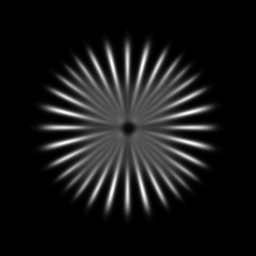
\includegraphics[scale=0.25]{Simulation deconvolution/ref_conv/RL_50.png}
		\\
		Fig.~\ref{fig:sim:ng0.1}                                                        &
		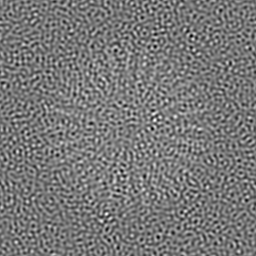
\includegraphics[scale=0.25]{Simulation deconvolution/ref_ng_0.1/RIF_0.01.png}  &
		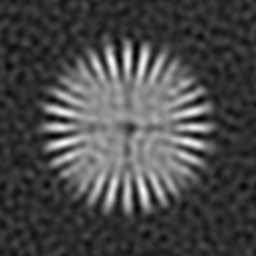
\includegraphics[scale=0.25]{Simulation deconvolution/ref_ng_0.1/RIF_1.png}     &
		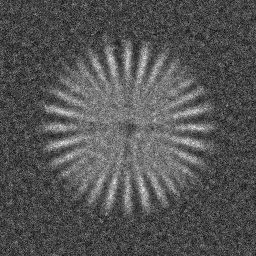
\includegraphics[scale=0.25]{Simulation deconvolution/ref_ng_0.1/RL_10.png}     &
		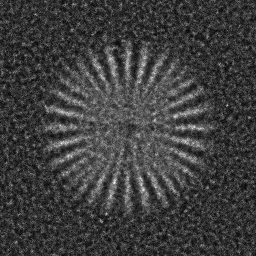
\includegraphics[scale=0.25]{Simulation deconvolution/ref_ng_0.1/RL_50.png}
		\\
		Fig.~\ref{fig:sim:ng0.01}                                                       &
		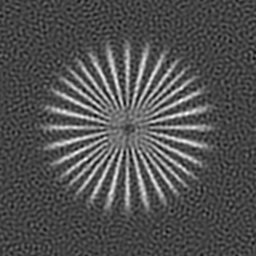
\includegraphics[scale=0.25]{Simulation deconvolution/ref_ng_0.01/RIF_0.01.png} &
		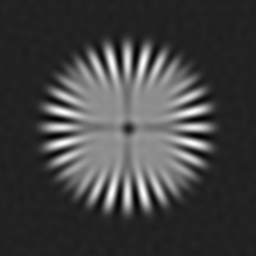
\includegraphics[scale=0.25]{Simulation deconvolution/ref_ng_0.01/RIF_1.png}    &
		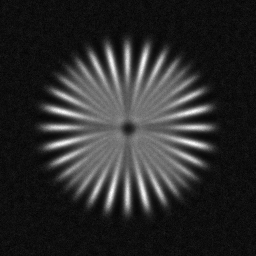
\includegraphics[scale=0.25]{Simulation deconvolution/ref_ng_0.01/RL_10.png}    &
		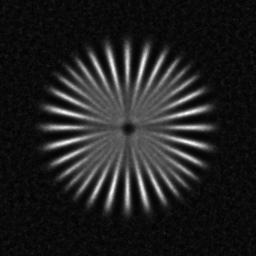
\includegraphics[scale=0.25]{Simulation deconvolution/ref_ng_0.01/RL_50.png}
		\\
		Fig.~\ref{fig:sim:np0.01}                                                       &
		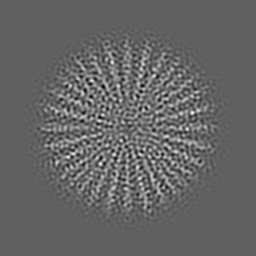
\includegraphics[scale=0.25]{Simulation deconvolution/ref_np_0.01/RIF_0.01.png} &
		
\includegraphics[scale=0.25]{Simulation deconvolution/ref_np_0.01/RIF_1.png}    &
		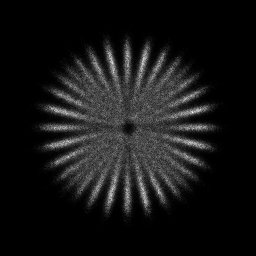
\includegraphics[scale=0.25]{Simulation deconvolution/ref_np_0.01/RL_10.png}    &
		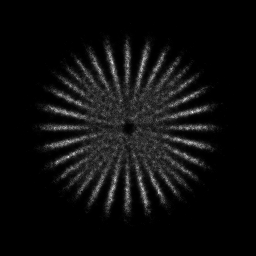
\includegraphics[scale=0.25]{Simulation deconvolution/ref_np_0.01/RL_50.png}
		\\
	\end{tabular}
	\caption{Matriz de los filtros realizados para recuperar las imágenes con ruido añadido simulado. Cada fila d se corresponde a una figura de \ref{fig:convolutions} (a--d), cada columna indica un método de recuperación}
\end{figure}


%%%%%%%%%% If using BibTeX:
\bibliography{bibliography}

\end{document}
